% ===============================================
% MATH 373: Intro to Numerical Analysis           Fall 2021
% prog5_testing_template.tex
% June 11, 2021
% ===============================================

% -------------------------------------------------------------------------
% You can ignore this preamble. Go on
% down to the section that says "START HERE" 
% -------------------------------------------------------------------------

\documentclass{article}

% load packages
\usepackage{amsmath,amsfonts,graphicx,amsthm,amssymb,hyperref,xcolor}

% Define default environments
\newenvironment{theorem}[2][Theorem]{\begin{trivlist}
\item[\hskip \labelsep {\bfseries #1}\hskip \labelsep {\bfseries #2.}]}{\end{trivlist}}
\newenvironment{lemma}[2][Lemma]{\begin{trivlist}
\item[\hskip \labelsep {\bfseries #1}\hskip \labelsep {\bfseries #2.}]}{\end{trivlist}}
\newenvironment{claim}[2][Claim]{\begin{trivlist}
\item[\hskip \labelsep {\bfseries #1}\hskip \labelsep {\bfseries #2.}]}{\end{trivlist}}
\newenvironment{problem}[2][Problem]{\begin{trivlist}
\item[\hskip \labelsep {\bfseries #1}\hskip \labelsep {\bfseries #2.}]}{\end{trivlist}}
\newenvironment{proposition}[2][Proposition]{\begin{trivlist}
\item[\hskip \labelsep {\bfseries #1}\hskip \labelsep {\bfseries #2.}]}{\end{trivlist}}
\newenvironment{corollary}[2][Corollary]{\begin{trivlist}
\item[\hskip \labelsep {\bfseries #1}\hskip \labelsep {\bfseries #2.}]}{\end{trivlist}}

\newenvironment{solution}{\begin{proof}[Solution]}{\end{proof}}

%adjust to 1 in margins
  \addtolength{\oddsidemargin}{-.875in}
   \addtolength{\evensidemargin}{-.875in}
    \addtolength{\textwidth}{1.75in}

    \addtolength{\topmargin}{-.875in}
    \addtolength{\textheight}{1.75in}
    
% Define Shortcuts
\def\ds{\displaystyle}
\def\beginrefs{\begin{list}%
        {[\arabic{equation}]}{\usecounter{equation}
         \setlength{\leftmargin}{2.0truecm}\setlength{\labelsep}{0.4truecm}%
         \setlength{\labelwidth}{1.6truecm}}}
\def\endrefs{\end{list}}
\def\bibentry#1{\item[\hbox{[#1]}]}

\begin{document}



% ------------------------------------------ %
%                 START HERE             %
% ------------------------------------------ %

\large

{\Large Math 373, Introduction to Numerical Analysis}

\begin{center}
{\Large Author: \hfill Amanda Lauen} % Replace "Author's Name" with your name
\end{center}
\par \medskip \par
{\Large Programming Assignment: 5} 
\par \bigskip \par

% Complete summary and remove the instructions in red
{\bf Summary:} {\color{black} The assignment calls for an initial value problem (IVP) to be solved using a MATLAB program.  This program takes in three inputs and outputs three values and a table (if applicable).  These three inputs are x0 (the initial starting position of the mass in meters), xp0 (the initial velocity of the mass in meters per second), and Tf (the length of time to run the model in seconds with time set at 0).  The model solved within this problem is the mass-spring system (the harmonic oscillator), represented in the following equation: $m\frac{d^2 x}{dt^2}+c\frac{dx}{dt}+kx=0$.  The initial values include m = 20 kg, k = 20 N/m, and c given by a piecewise function of values ranging from $t < 0$ to $t > 0$.  This problem is solved using the function ode23 explained in Dr. Kyle Riley’s lectures [KR21] and on the official MATLAB help site [Matlab].} 
\par \bigskip \par

% Complete methods and remove the instructions in red
{\bf Methods:} {\color{black} The possible outcome for this mathematical problem is a differential equation that satisfies the initial conditions given within the problem and validates the problem it solves.  The possible outcomes of running the program are a flag value, an array value of T, and a two-column array value W.  For array W, one column represents the values of the position for every time step.  The other column represents the velocity of the mass at every time step.  
\par \medskip \par
There are two flags to indicate if the program was executed correctly or not.  The first flag, flag 0, represents that the program did run successfully.  The second flag, flag 1, denotes that the input values given are not feasible, leading T and W to equal -9 in the process.  
The way that I made my code efficient was by testing that the code was producing accurate calculations.  To do this, I compared the results of my code with the analytical answer.  More on this verification is highlighted in the Testing and Analysis section and the Appendix section of this report.
\par \medskip \par
This problem can be solved analytically.  Though it can be solved analytically for $t > 0$ and $t < 10$, it is hard for $0\leq t<10$.  It depends on where you are in the system to see if it could be solved analytically.  In other words, you can do it for parts of the problem but not for the entirety of the problem.
 }
\par \bigskip \par


% Complete testing and analysis, please remove the instructions in red
{\bf Testing and Analysis:} {\color{black} I tested my program by first representing the system as first-order ordinary differential equations and validating it with the analytical answer.  By testing my program this way, I validated it by setting a constant c value and compared it to the analytical solution.  I did this by finding $mr^2+cr+k=0$.  This equation is a quadratic algebraic equation and can be solved using the MATLAB command “roots” to solve for r.  Hypothetically, the found values for r are $r_{1}$ and $r_{2}$. Therefore, a general solution to this problem is as follows: $x(t)=c_{1}e^{r_{1}t}+c_{2}e^{r_{2}t}$.  To find the values of the unknown constants in the following solution, I used the initial values given in the problem and wrote them in the following matrix: $\begin{bmatrix}
1 & 1\\ 
 r_{1}& r_{2} 
\end{bmatrix}
\begin{bmatrix}
c_{1}\\ 
c_{2}
\end{bmatrix}=\begin{bmatrix}
x_{0}\\ 
v_{0}
\end{bmatrix}$.  
By doing this, the MATLAB "$\backslash$" operator can solve this matrix system.  Included in this program is a MATLAB document called cmprWithAnal.m, which calculates the above work.  More details about testing and validation will be highlighted further in the Appendix section of this report.
\par \medskip \par
I handled the variation in the value of c for solving the initial value problem by creating another function and using if statements to run the code for that time t.  This function was from the modified \textunderscore euler  \textunderscore sys.m file created by Dr. Kyle Riley [KR21].  This function evaluated F(t, W) for the initial value problem in a first-order system form.  Doing this creates and figures out which c value to use, but it also helps with the assigned unit.  Since each term in the system equation, $mx''+cx'+kx=0$, is a force value, the c value must have the same force units.  Hence, the units of c are N (Newtons) per meters per second (N/(m/s)).
This variation of c does not present issues with the accuracy of the results.
\par \medskip \par
The results would be more accurate if the program used ode45 instead of ode23.  The reason being is that ode45 has a higher predictor and corrector than ode23, meaning more accuracy.  Though this may be the case, more work per iteration happens in ode45, leading to a higher convergence.  With this, tolerance must be considered to see if this all applies.  If the tolerance is the same, then the above statements do not apply.  If different, then it would change accordingly.  Accuracy for ode23 and ode45 depends on tolerance, and if there is something different in the tolerance, then the accuracy of both functions will be changed.
 
}
\par \bigskip \par

%Hit list is optional, but is evidence of higher learning, developing strong skills in reviewing are extremely valuable. Please remove instructions in red.
{\bf Hit List: }{\color{black} When writing this report, there are not any missing or known problems with my program that I know of.  If I had more time, I would have liked to know how many systems we could have tested before the code would not work anymore.  It would have been interesting to know the limit of this code and how much it could do before we got a NaN error or an Inf error.
}
\par \bigskip \par

%Integrity Statement Leave the statement in red and follow it with ``I affirm that this program submission complies with the integrity specifications of this assignment. I understand if I am in violation of the integrity specification then I will get a zero on the assignment and receive an overall reduction in my course grade by one letter grade. ``

{\bf Academic Integrity}: {\color{black} The goal of this assignment is that everyone write their own code. This means you should not copy any code from any other source (the only exception are the templates provided by the instructor.) If you copy any code then you are in violation of integrity specifications of this assignment. If you provide your code to others then you are also in violation of the integrity rules of this assignment.
\par \medskip \par
I affirm that this program submission complies with the integrity specifications of this assignment. I understand if I am in violation of the integrity specification then I will get a zero on the assignment and receive an overall reduction in my course grade by one letter grade.}


% Add references here, list alphabetically according to last name of primary author.
\section*{References}
\beginrefs

\bibentry{Matlab} {\sc Matlab website}, \href{https://www.mathworks.com}{www.mathworks.com}, August 2019. % put exact and full link in the first listing right after href

\bibentry{KR21} {\sc Kyle Riley}, Class Lecture, Math 373: Introduction to Numerical Analysis, Lecture, August 2021. 

\endrefs

\bigskip \par \bigskip
%%%------------------------------------------------------
%  Appendix, remove the red comments when completing this section. 
%%----------------------------------------------------------
{\Large {\bf Appendix}} \par \medskip

{\color{black} As stated in the Testing and Analysis portion of this report, I tested my program by representing the system as a system of first-order ordinary differential equations.  To do this, I chose the following variables $w_{1}$ and $w_{2}$, to represent x and x’ ($\frac{dx}{dt}$) respectively.  That is:
\par \medskip \par
$w_{1}=x$
\par \medskip \par
$w_{2}=x'$
\par \medskip \par
Now we can write the following:
\par \medskip \par
$w_{1}'=x'=w_{2}$  
\par \medskip \par
$w_{2}'=x''=-(\frac{c}{m})x'-(\frac{k}{m})x=-(\frac{c}{m})w_{2}-(\frac{k}{m})w_{1}$
\par \medskip \par
So, what we can use in the coding is as below: 
\par \medskip \par
$w_{1}'=w_{2}$ 
\par \medskip \par
$w_{2}'=-(\frac{c}{m})w_{2}-(\frac{k}{m})w_{1}$
\par \medskip \par
In order to validate that my program is producing an accurate calculation, we can set a constant value for “c” and get results and compare it with the analytical answer: $mx''+cx'+kx=0$. 
\par \medskip \par
Suppose the answers are exponential functions $x=e^{rt}$ with unknown parameter r, by substation in the ODE, we find that: $mr^2+cr+k=0$.  
\par \medskip \par
This equation is a quadratic algebraic equation, and we can solve it using MATLAB command “roots” to find the values of r; suppose they found values are $r_{1}$ and $r_{2}$. Therefore, we can write the general solution of the ODE as $x(t)=c_{1}e^{r_{1}t}+c_{2}e^{r_{2}t}$.
\par \medskip \par
To find the values of the unknown constants in the above solution, we use the initial value of the problem: 
\par \medskip \par
$x'(t)=c_{1}e^{r_{1}t}+c_{2}e^{r_{2}t}$
\par \medskip \par
$x(0)=c_{1}+c_{2}=x_{0}$
\par \medskip \par
$x'(0)=c_{1}r_{1}+c_{2}r_{1}=v_{0}$
\par \medskip \par
The above equations are a system of linear equations, and we can write them in the following matrix form:
\par \medskip \par
$\begin{bmatrix}
1 & 1\\ 
 r_{1}& r_{2} 
\end{bmatrix}
\begin{bmatrix}
c_{1}\\ 
c_{2}
\end{bmatrix}=\begin{bmatrix}
x_{0}\\ 
v_{0}
\end{bmatrix}$.  
\par \medskip \par
This system of linear equations can be solved using the MATLAB "$\backslash$" operator.
\par \medskip \par
The script “cmprWithAnal.m” is provided to do the above calculations and superimpose the time response of the analytic method with the numerical method used in my original program.  In order to run the given script, a constant “c” must be set in proge820474.m, furthermore, all input data in both codes must be the same. The constant c value is commented out in proge820474.m for this case.  After running the script “cmprWithAnal,” the following chart is printed.  This chart is shown in Figure 1 on the following page:
\par \medskip \par
 \begin{figure}[!ht]
\centering  %centering can be used to center the image
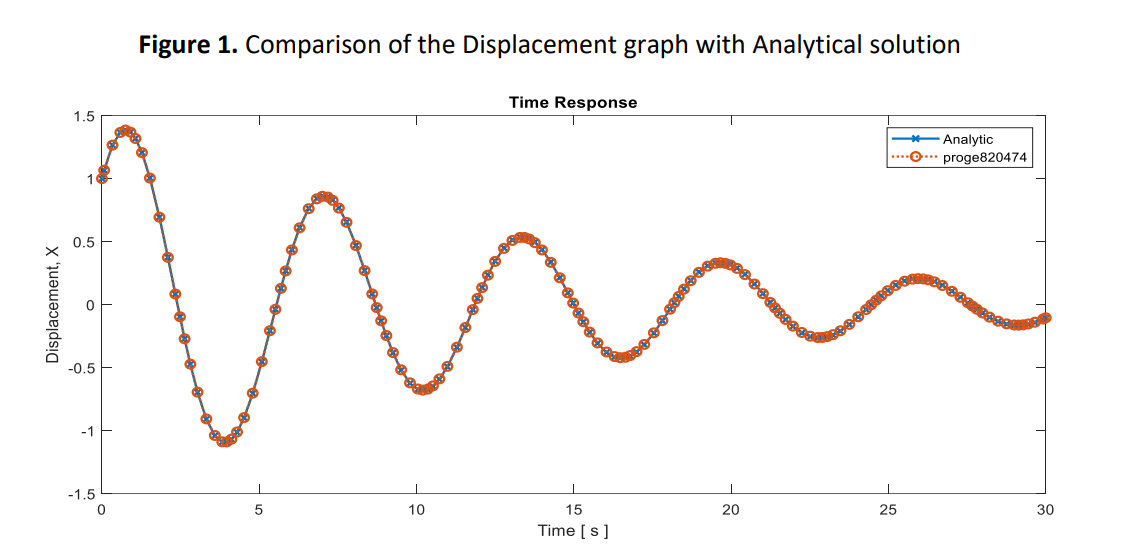
\includegraphics[height=75mm]{Programs/Program 5/proge820474fig1.PNG}
 \caption{Comparison of the Displacement Graph with the Analytical Solution}
 \label{f:Graph 1}
\end{figure}
\par \medskip
\par \bigskip \par
\par \bigskip \par
\par \bigskip \par
\par \bigskip \par
\par \bigskip \par
\par \bigskip \par
\par \bigskip \par
\par \bigskip \par
\par \bigskip \par
\par \bigskip \par
\par \bigskip \par
\par \bigskip \par
\par \bigskip \par
\par \bigskip \par
\par \bigskip \par
\par \bigskip \par
\par \bigskip \par
\par \bigskip \par
\par \bigskip \par
\par \bigskip \par
\par \bigskip \par
\par \bigskip \par
These results show that the numerical solution of the system implemented in proge820474.m has a very good match with the analytical solution; hence it is a valid code to deal with the provided initial value problem (IVP). 
\par \medskip \par
Since this is a damped case of free vibration of a single degree of freedom (DOF), we expect it behaves like a damped single degree of freedom vibrating system.  In other words, the time response should oscillate and dampen gradually as it moves along. To verify this, I called the function with the following command in the MATLAB command window:
\par \medskip \par
$>> [flag, T, W] = proge820474(80,1,0.8);$
\par \medskip \par
A note on the printed answers below: the matrices T and W were shortened to show the first four terms within their respective matrices (4 x 1 and 4 x 2 matrices) to save space on this document.  The reason for this is that the actual results are 375 x 1 and 375 x 2 matrices.  The following code below represents these changes and the results of the code above being run along with Figure 2 being represented on the following page:
\par \medskip \par
$flag = 0$
\par \medskip \par
$T = \begin{bmatrix}
0\\ 
0.0552\\ 
0.3030\\ 
0.5405
\end{bmatrix}$
\par \medskip \par
$W = \begin{bmatrix}
1.0000 & 0.8000\\ 
 1.0424& 0.7352\\ 
 1.1867& 0.4285\\ 
 1.2522& 0.1243
\end{bmatrix}$
\par \medskip \par
 \begin{figure}[!ht]
\centering  %centering can be used to center the image
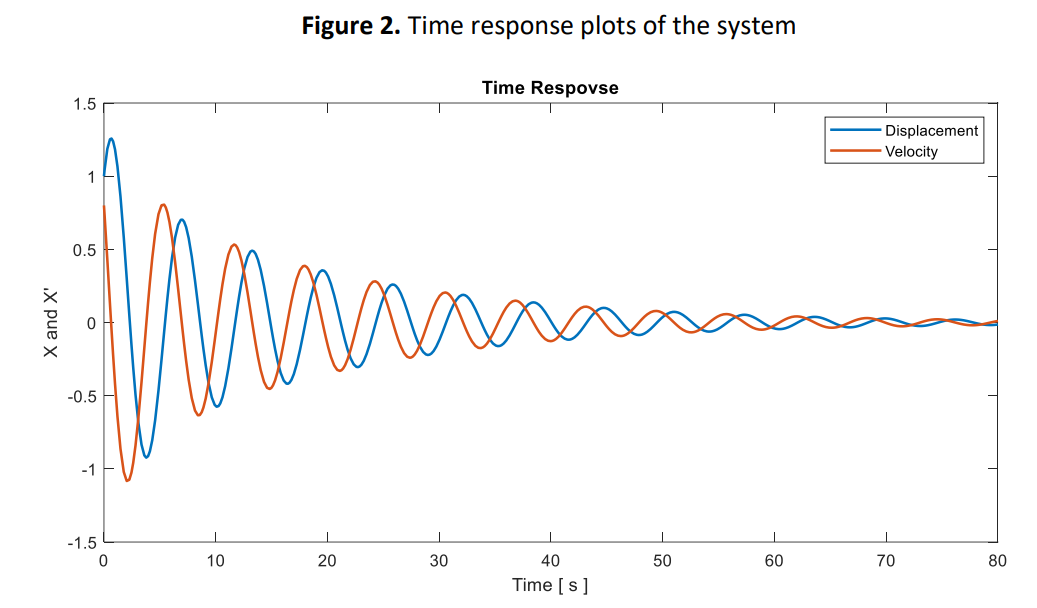
\includegraphics[height=75mm]{Programs/Program 5/proge820474fig2.PNG}
 \caption{Time Response Plots of the Given System}
 \label{f:Graph 2}
\end{figure}
\par \medskip
\par \bigskip \par
\par \bigskip \par
\par \bigskip \par
\par \bigskip \par
\par \bigskip \par
\par \bigskip \par
\par \bigskip \par
\par \bigskip \par
\par \bigskip \par
As shown in Figure 2 above, the time response is what we expected.  
\par \medskip \par
To test edge cases, I used the try and catch statement.  The “try, catch” statement is a statement that allows you to execute statements and catch resulting errors if there are any [Matlab].  It allows the code to run even when faced with an error but provides the error message in a variable named “me.”  I used this statement to catch any error that may not be listed within the code, i.e., any error inside “ode23” for any reason.  
\par \medskip \par
Flag 1 can be printed when you enter in the wrong arguments.  One example includes the following code:
\par \medskip \par
$>> [flag, T, W] = proge820474(-10,1,0.8);$
\par \medskip \par
The following results are printed within the Command Window:
\par \medskip \par
$flag = 1$
\par \medskip \par
$T = -9$
\par \medskip \par
$W =  -9$
\par \medskip \par
As shown above, whenever a user enters invalid inputs, the correct flag prints. The entry of letters, a 0 value for Tf, or brackets around specific values also prints the error flag of 1.  
\par \medskip \par
From the above example call functions, I concluded that:
\par \medskip \par
1.	Comparing the program outputs with the analytical value found in cmprWithAnal.m shows that the numerical solution of the system implemented is valid to deal with the provided IVP.
\par \medskip \par
2.	The code provides the desired results when the input values Tf, x0, and xp0 are not feasible.
\par \medskip \par
3.	When the input values are valid, the values of flag, T, and W are represented, and a plot is printed, respectively.
\par \medskip \par
Thus, the code and the calculations validation with the analytical answer prove that the program produces accurate calculations.
} 
\par \medskip

% ---------------------------------------------------
% Anything after the \end{document} will be ignored by the typesetting.
% ----------------------------------------------------

\end{document}